% !TEX root = ../main.tex

\chapter{注意力蒸馏方法对基准模型的改进}

我们在第\ref{chap:baseline_model}章讨论了3D-UNet网络这一基准模型对支气管气道树的分割, 仔细观察表\ref{tbl:visualize_airway_3d_model}
中各个支气管气道树末端(ATM\_174\_0000和ATM\_505\_0000两个病例除外)出现很多红色的假阴性支气管体素,见图\ref{fig:distal_bronchus}
中放大的左右末梢支气管。假阴性表示这些体素原本是真实存在的支气管体素,只是因为我们的3D-UNet基准网络的分割能力不够,尚无足够的精细分割能力。
\begin{figure}[!htp]
    \centering
    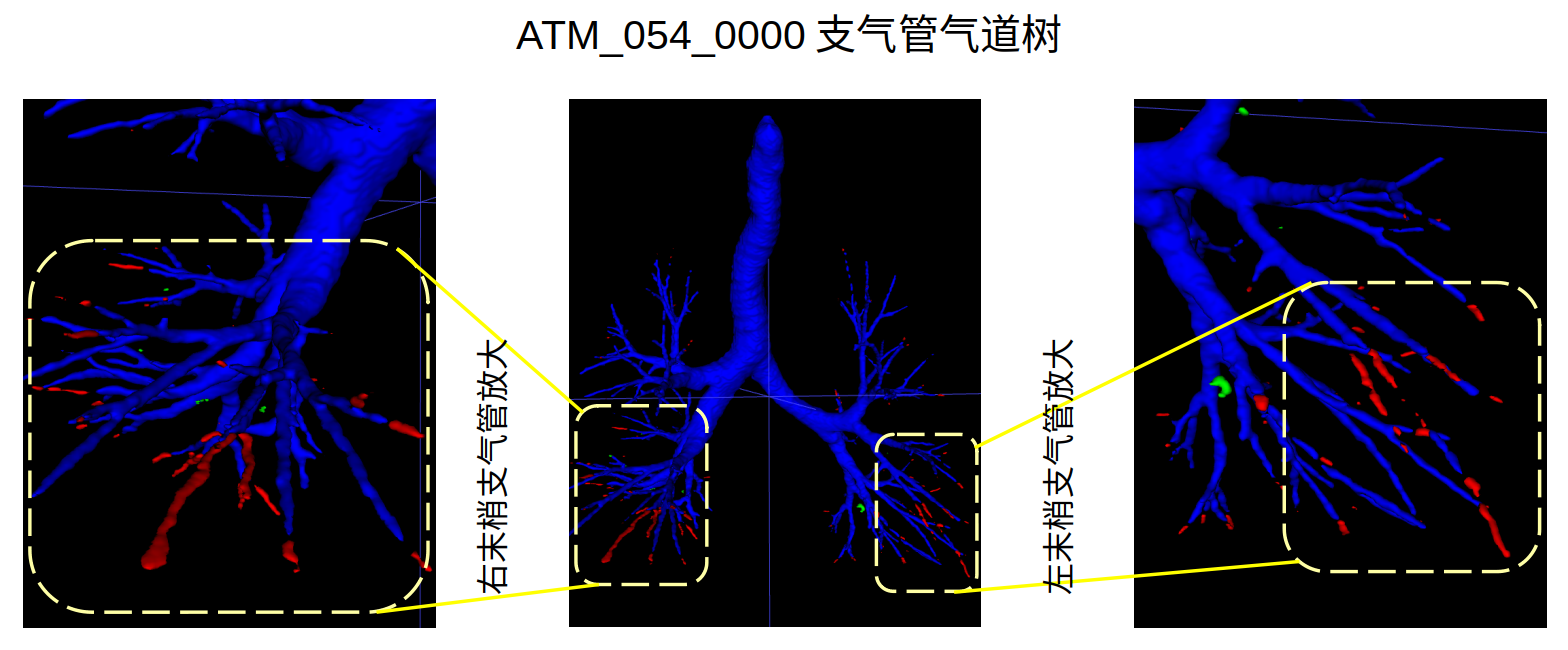
\includegraphics[width=\textwidth]{zoom_in_distal_bronchus}
    \bicaption[末梢支气管出现假阴性分割效果]
        {末梢支气管出现假阴性分割效果}
        {The distal bronchus segmentation showed false-negative voxels}
    \label{fig:distal_bronchus}
\end{figure}
末梢支气管的管径通常都比较小,做标注工作的临床医生在标注这些末梢支气管尽很大的努力,可能只能看到一到两个像素。ATM\_054\_0000切片上
的像素间距是0.83mm,切片间距是0.5mm,由此可见末端支气管的管径在人体肺部实际不到1mm。 对于医生来说,精细标注确实是一个比较大
的挑战,大量CT图片的精细标注是一项繁重耗时且枯燥乏味的工作。但对于支气管镜导航手术来说,越是进入末梢支气管越能接近肺癌结节
部位,越好做到微创甚至无创取样活检。这就要求我们做支气管气道树分割越精细越好,较高要求是能分割到段支气管。当然最高要求是做到
能分割小叶支气管,小叶支气管是最末端的毛细支气管,直接连到肺泡。

对于卷积网络提取精细特征的要求,Sergey Zagoruyko等人\cite{Zagoruyko2016PayingMA}提出卷积网络注意力转移Attention Transfer
的方法,注意力转移将知识从教师网络转移到学生网络,可以改善CNN的分割性能。 Geoffrey Hinton和Jeff Dean等人\cite{Hinton2015DistillingTK}
提出知识蒸馏的概念,指出注意力图是一种有价值的知识。受此启发,知识可迁移,注意力帮助聚焦,我们提出注意力蒸馏的方法。在学习支气管
气道树的特征时,加强对末梢支气管这些细小对象的关注,可帮助提高3D-UNet网络的分割性能。

\section{注意力蒸馏方法}

注意力是一组空间地图,本质是试图使网络在做出输出决策时最关注的输入空间区域\cite{Zagoruyko2016PayingMA}。有两种注意力图
的形式,一种是基于激活的注意力图Activation-based attention map, 另一种是基于梯度的注意力图Gradient-based 
attention map. 这种注意力图可在网络的各个层定义,以便它们能够捕获低级、中级和高级别的表示信息。注意力图可指导我们看哪里,
把目光聚焦在感兴趣的地方。 

在卷积网络的第$n$层,定义注意力图${AttMap}_{n}$作用在该层特征${Feat}_{n}$的函数关系:
\begin{equation}\label{eq:attention_map}
    \mathcal{F}: {Feat}_{n}^{C \times D \times H \times W} \longrightarrow {AttMap}_{n}^{1 \times D \times H \times W}
\end{equation}
这里上标$D \times H \times W$表示维数,因为3D-UNet是以三维长方体子块体数据为输入的,就像UNet以二维的图像数据为输入的。
二维图像数据的维度是$Height \times Width$,三维长方体子块体数据的维度是$Depth \times Height \times Width$。而$C$
表示通道维数,也就是在第$n$层卷积有$C$个$D \times H \times W$个长方体子块。

如何计算\ref{eq:attention_map}式的函数关系? Sergey Zagoruyko等人在论文\textit{Paying more attention to Attention: 
Improving the performance of convolutional neural networks via Attention Transfer}中提出了三种计算方式
\cite{Zagoruyko2016PayingMA}:
\begin{enumerate}
    \item 沿着通道维数,计算绝对值之和  
    \begin{equation}
        \mathcal{F}_{sum}({Feat}_{n}) = \sum_{c=1}^{C}{\left\lvert {Feat}_{n} \right\rvert}
    \end{equation}
    
    \item 沿着通道维数,计算绝对值的$p$次幂之和
    \begin{equation}
        \mathcal{F}_{sum}^{p}({Feat}_{n}) = \sum_{c=1}^{C}{\left\lvert {Feat}_{n} \right\rvert}^{p}
    \end{equation}
    
    \item 沿着通道维数,计算绝对值的$p$次幂的最大值
    \begin{equation}
        \mathcal{F}_{max}^{p}({Feat}_{n}) = {max}_{c=1}^{C}{\left\lvert {Feat}_{n} \right\rvert}^{p}
    \end{equation}
\end{enumerate}
在这里我们选择第2种计算方式,沿着通道维数,计算绝对值的$p$次幂之和。因为这种计算方式保留了该层特征的所有隐含的显著激活信息,
但不会忽略非最大的元素,也不会削弱判别性的元素。$p$次幂建议取$p = 2$, 它增强了大多数敏感任务区域。$\mathcal{F}_{sum}^{p}({Feat}_{n})$
的计算相比于$\mathcal{F}_{sum}({Feat}_{n})$,它把更多的权重放置于最具判别性的部位。$p$越大,越能聚焦于这些判别性部位。

借助于PyTorch的张量表示方法,我们将注意力图函数改写成如下形式:
\begin{equation}
    {AttMap}_{n} = \mathcal{F}_{sum}^{p}(Feat_{n}) = \sum_{c=1}^{C}{\left\lvert {Feat}[c, :, :, :] \right\rvert}^{p}
\end{equation}
其中$Feat[c, :, :, :]$表示通道维$c$、 深度维$D$、 高度维$H$、宽度维$W$, 后面的$[:, :, :]$就构成了一个$D \times H \times W$的
长方体子块。

这种计算注意力图的方式其意义就是将$C$个$D \times H \times W$长方体子块的特征信息蒸馏浓缩在一个$D \times H \times W$长方体
子块特征里。如图\ref{fig:attention_distillation}所示:
\begin{figure}[!htp]
    \centering
    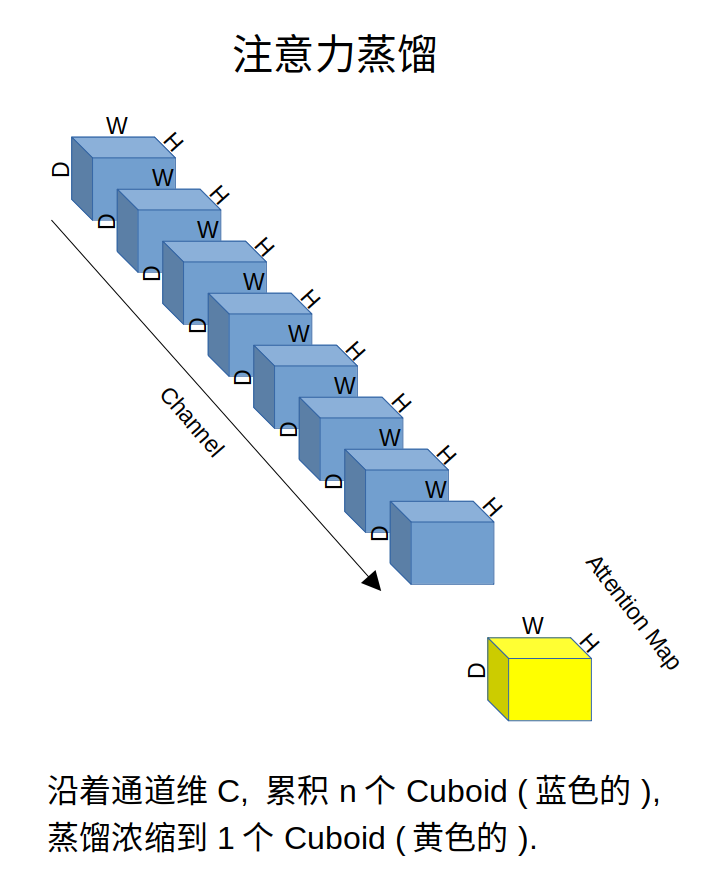
\includegraphics[width=0.6\textwidth]{Attention_Distillation}
    \bicaption[注意力蒸馏的原理]
        {注意力蒸馏的原理}
        {How the attention distillation works}
    \label{fig:attention_distillation}
\end{figure}

为了保证蒸馏得到的注意力图Cuboid与原来的特征Cuboid保持相同的$D \times H \times W$维数,我们需要对注意力图进行三线性
插值Trilinear Interpolation $\mathcal{L}(\bullet)$
\begin{equation}
    {AttMap}_{n} = \mathcal{L}\left[\mathcal{F}_{sum}^{p}(Feat_{n})\right]
\end{equation}

最后,我们使用$Softmax$对其归一化,使每个体素的值被限定在$[0, 1]$之间。
\begin{equation}
    {AttMap}_{n} = {Softmax}\{ \mathcal{L}\left[\mathcal{F}_{sum}^{p}(Feat_{n})\right] \}
\end{equation}

注意力图的引入给卷积网络的层与层之间相当于增加里一个额外的梯度,使相邻两层之间更接近,可以使${AttMap}_{n}$与${AttMap}_{n+1}$
之差最小化,即它们的累积损失最小。
\begin{equation}
    Loss = min \sum_{n=1}^{N-1}\lVert {AttMap}_{n} - {AttMap}_{n+1} \rVert_{F}^{2}
\end{equation}
其中$\lVert \bullet \rVert_{F}$是指矩阵的Frobenius范数。

以上是注意力图的计算过程。引入注意力蒸馏的目的是为了增加对细颗粒度的物体的关注,在本文中就是为了增加对末梢支气管这些细小的支气管
体素的关注,从而提高分割的性能。

\section{注意力蒸馏的效果可视化}

引入注意力蒸馏方法后,我们可以来看看在卷积网络不同层之间,经过蒸馏后特征的表现如何? 通过可视化的方式来查看支气管气道树。

